
%(BEGIN_QUESTION)
% Copyright 2010, Tony R. Kuphaldt, released under the Creative Commons Attribution License (v 1.0)
% This means you may do almost anything with this work of mine, so long as you give me proper credit

Anta at denne temperaturmålekretsen feilaktig viser svært lav temperatur (full nedskala) når RTD-sensoren faktisk måler romtemperatur (20 $^{o}$C). Et digitalt multimeter (DMM) koblet mellom testpunktene {\bf A} og {\bf C} viser 1 volt:

$$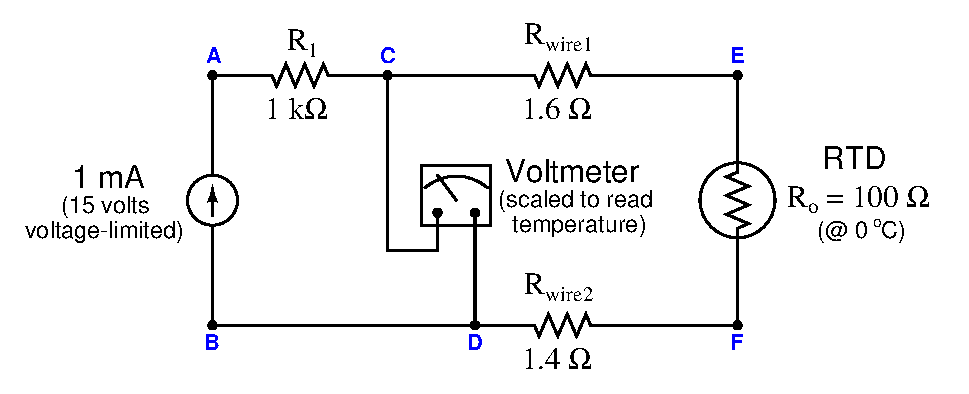
\includegraphics[width=15.5cm]{i00804x01.eps}$$

Vurder sannsynligheten for hver oppgitt feil i denne kretsen. Betrakt én feil om gangen (dvs. ingen samtidige feil), og avgjør om hver feil alene kan forklare {\it alle} målinger og symptomer i kretsen.

% No blank lines allowed between lines of an \halign structure!
% I use comments (%) instead, so that TeX doesn't choke.

$$\vbox{\offinterlineskip
\halign{\strut
\vrule \quad\hfil # \ \hfil & 
\vrule \quad\hfil # \ \hfil & 
\vrule \quad\hfil # \ \hfil \vrule \cr
\noalign{\hrule}
%
% First row
{\bf Feil} & {\bf Mulig} & {\bf Umulig} \cr
%
\noalign{\hrule}
%
% Another row
$R_1$ avbrutt &  &  \cr
%
\noalign{\hrule}
%
% Another row
Voltmeter avbrutt &  &  \cr
%
\noalign{\hrule}
%
% Another row
Leder 1 avbrutt &  &  \cr
%
\noalign{\hrule}
%
% Another row
Leder 2 avbrutt &  &  \cr
%
\noalign{\hrule}
%
% Another row
RTD avbrutt &  &  \cr
%
\noalign{\hrule}
%
% Another row
$R_1$ kortsluttet &  &  \cr
%
\noalign{\hrule}
%
% Another row
Voltmeter kortsluttet &  &  \cr
%
\noalign{\hrule}
%
% Another row
RTD kortsluttet &  &  \cr
%
\noalign{\hrule}
%
% Another row
Strømkilde død &  &  \cr
%
\noalign{\hrule}
} % End of \halign 
}$$ % End of \vbox

Til slutt: angi {\it neste} diagnostiske test eller måling du ville gjort på systemet. Forklar hvordan resultatet av denne testen hjelper videre med å avdekke feilens plassering og/eller art.

\vfil 

\underbar{file i00804}
\eject
%(END_QUESTION)





%(BEGIN_ANSWER)


%(END_ANSWER)





%(BEGIN_NOTES)

% No blank lines allowed between lines of an \halign structure!
% I use comments (%) instead, so that TeX doesn't choke.

$$\vbox{\offinterlineskip
\halign{\strut
\vrule \quad\hfil # \ \hfil & 
\vrule \quad\hfil # \ \hfil & 
\vrule \quad\hfil # \ \hfil \vrule \cr
\noalign{\hrule}
%
% First row
{\bf Feil} & {\bf Mulig} & {\bf Umulig} \cr
%
\noalign{\hrule}
%
% Another row
$R_1$ avbrutt &  & $\surd$ \cr
%
\noalign{\hrule}
%
% Another row
Voltmeter avbrutt & $\surd$ &  \cr
%
\noalign{\hrule}
%
% Another row
Leder 1 avbrutt &  & $\surd$ \cr
%
\noalign{\hrule}
%
% Another row
Leder 2 avbrutt &  & $\surd$ \cr
%
\noalign{\hrule}
%
% Another row
RTD avbrutt &  & $\surd$ \cr
%
\noalign{\hrule}
%
% Another row
$R_1$ kortsluttet &  & $\surd$ \cr
%
\noalign{\hrule}
%
% Another row
Voltmeter kortsluttet & $\surd$ &  \cr
%
\noalign{\hrule}
%
% Another row
RTD kortsluttet & $\surd$ &  \cr
%
\noalign{\hrule}
%
% Another row
Strømkilde død &  & $\surd$ \cr
%
\noalign{\hrule}
} % End of \halign 
}$$ % End of \vbox

En god ``neste test'' er å måle spenning over voltmeteret eller over RTD-terminalene.




\vskip 20pt \vbox{\hrule \hbox{\strut \vrule{} {\bf Virtual feilsøking} \vrule} \hrule}

Denne oppgaven egner seg godt som ``Virtual feilsøking''. Presenter diagrammet for studentene, tenk deg først en bestemt feil i systemet, og presenter deretter ett eller flere symptomer på denne feilen. Studentene foreslår så diagnostiske tester for å finne feiltype og plassering, som om de faktisk feilsøker anlegget. Din oppgave er å oppgi hvilke resultater disse testene ville gitt, og dokumentere dem synlig for alle.

Under og etter øvelsen er det nyttig å stille oppfølgingsspørsmål som:

\begin{itemize}
\item{} Hva forteller resultatet av siste diagnostiske test om feilen?
\item{} Hvis resultatet av siste test hadde vært annerledes, hva ville det fortalt om feilen da?
\item{} Er siste diagnostiske test den beste testen vi kunne gjort?
\item{} Hva ville vært ideell testrekkefølge for å finne feilen på færrest mulig trinn?
\end{itemize}


%INDEX% Troubleshooting review: electric circuits

%(END_NOTES)
